\documentclass{article}
\usepackage{amsfonts}
\usepackage{amsmath}
\usepackage{hyperref}
\usepackage{tikz}
\usepackage{subcaption}
\usepackage{siunitx}
\usepackage[nottoc]{tocbibind}
\usepackage{xeCJK}
\usepackage{soul}
\usepackage{datetime}
\usepackage[a4paper, total={7in, 10in}]{geometry}

\newdateformat{chinesedate}{\THEYEAR 年\THEMONTH 月\THEDAY 日}

\usetikzlibrary{decorations.pathreplacing}

\providecommand{\keywords}[1]
{
  \small	
  \textbf{\textit{Keywords---}} #1
}

\title{Self-supervised hamiltonian mechanics neural networks}
\author{詹有丘 (Youqiu Zhan)}

\begin{document}

\Huge

~\par
~\par
\noindent 参赛队员姓名:\underline{詹有丘}\par
~\par
\noindent 中学:\underline{上海交通大学附属中学}\par
~\par
\noindent 省份:\underline{上海市}\par
~\par
\noindent 国家/地区:\underline{中国}\par
~\par
\noindent 指导教师姓名:\underline{~~~}\par
~\par
\noindent 论文题目:\ul{A multifunctional hamiltonian mechanics simulator and some of its application examples}

\newpage

\huge

~\par
~\par
\setlength{\parindent}{5ex}
本参赛团队声明所提交的论文是在指导老师指导下进行的研究工作和取得的研究成果。尽本团队所知,除了文中特别加以标注和致谢中所罗列的内容以外,论文中不包含其他人已经发表或撰写过的研究成果。若有不实之处,本人愿意承担一切相关责任。\par
~\par
~\par
参赛队员:\underline{詹有丘}\qquad 指导老师:\underline{~~~}\par
~\par
\begin{flushright}\chinesedate\today\end{flushright}

\normalsize

\setlength{\parindent}{1.5em}

\maketitle

\begin{abstract}
TBD
\end{abstract}

\keywords{hamiltonian, machine learning, mechanics}

\tableofcontents

\section{Introduction}

When one observes the motion of a system,
he may be curious about what is the hamiltonian of it
if such a hamiltonian exists.

Here there have been several approaches to do this,
such as the hamiltonian neural network \cite{greydanus2019hamiltonian},
the lagrangian neural network \cite{cranmer2020lagrangian},
and the neural ODE \cite{chen2018ode}.
Like what we are going to do,
they optimize a neural network that reads the state $\mathbf x$ of a system as the input
and outputs the change of state w.r.t. time $\mathrm d\mathbf x/\mathrm dt$ of the system.

In this process, they have a common property:
they train the neural network in a supervised mode,
which means there are $\mathrm d\mathbf x/\mathrm dt$ ground truth in the dataset.
However, in a physics experiment, measuring the change rate of the state is probably more difficult than directly measuring the state.
Thus, we want to introduce a method to optimize the neural network in a self-supervised way.

\section{Canonical equation and ODE}

To build a common sense of the physics theories it is going to involve,
the canonical equation is introduced.

The canonical equation is a set of ordinary differential equations (ODE)
whose solution depicts the motion of the system.
The equation in mathematical form is \cite{hand2008mechanics}\cite[p. 65]{arnold1989mathmech}\cite[p. 132]{landau1976mechanics}
\begin{equation}
	\dot{\mathbf q}=\frac{\partial\mathcal H}{\partial\mathbf p},
	\quad
	\dot{\mathbf p}=-\frac{\partial\mathcal H}{\partial\mathbf q},
	\label{eq:canonical}
\end{equation}
where $\mathbf q\in\mathbb R^n$ is the \textbf{generalized coordinates},
$\mathbf p\in\mathbb R^n$ is the \textbf{generalized momentum},
and $\mathcal H$ is the \textbf{hamiltonian} of the system,
which is a scalar function w.r.t. $t$, $\mathbf q$, and $\mathbf p$.
$n$ is the number of degrees of freedom (DOF).
A hamiltonian is specific for a specific system.

The tuple $\mathbf x:=\left(\mathbf q,\mathbf p\right)\in\mathbb R^{2n}$
is called the \textbf{canonical coordinates}.
In computer programs, it is convenient to write Equation \ref{eq:canonical}
in form of
\begin{equation}
	\dot{\mathbf x}=\mathbf f\left(t,\mathbf x\right),
\end{equation}
which is the common form of ODE.
Here in our specific case,
\begin{equation}
	\mathbf f\left(t,\mathbf x\right):=\boldsymbol\omega\nabla_{\mathbf x}\mathcal H,
	\label{eq:ode}
\end{equation}
where the notion $\boldsymbol\omega\nabla_{\mathbf x}$ denotes the \textbf{symplectic gradient} w.r.t. $\mathbf x$,
whose first $n$ components is the gradient w.r.t. the last $n$ components of $\mathbf x$,
and the last $n$ components is the negative gradient w.r.t. the first $n$ components of $\mathbf x$.

One of properties of the symplectic gradient is that,
moving along the symplectic gradient field of a scalar does not change the value of the scalar function,
which means that the value of $\mathcal H$ is conserved if $\partial\mathcal H/\partial t=0$ \cite[p. 67]{arnold1989mathmech}\cite[p. 132]{landau1976mechanics}.
In fact, the physical meaning of $\mathcal H$ is the energy,
so its conservation is obvious.

According to Equation \ref{eq:ode}, the difference between $\mathbf x$ at 2 different times is an integral
\begin{equation}
	\mathbf x\left(t_2\right)=\mathbf x\left(t_1\right)+\int_{t_1}^{t_2}\mathbf f\left(t,\mathbf x\left(t\right)\right)\mathrm dt.
	\label{eq:int}
\end{equation}
The integral can be calculated using the \href{https://github.com/rtqichen/torchdiffeq}{torchdiffeq} Python package \cite{chen2018ode}.

\begin{figure}[h!]
	\centering
	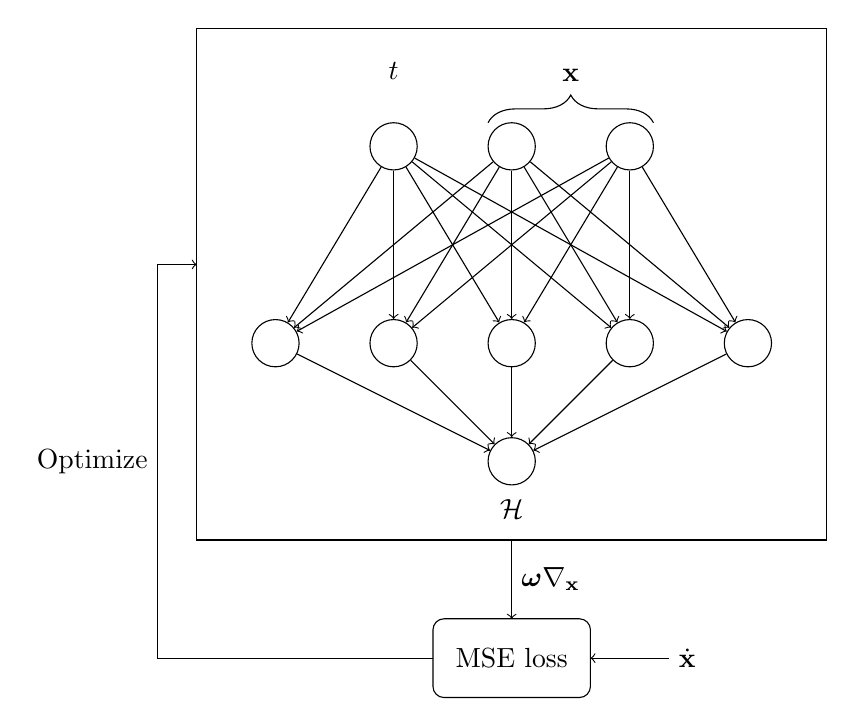
\begin{tikzpicture}
		\tikzstyle{neuron}=[circle,draw=black,minimum size=0.6cm,inner sep=0]
		\foreach \x in {-1,...,1}
			\node[neuron] (input\x) at (1.5*\x, 0) {};
		\foreach \x in {-2,...,2}
			\node[neuron] (hidden\x) at (1.5*\x, -2.5) {};
		\node[neuron] (output) at (0, -4) {};

		\foreach \xin in {-1,...,1}
			\foreach \xout in {-2,...,2}
				\path[->] (input\xin) edge (hidden\xout);
		\foreach \xin in {-2,...,2}
			\path[->] (hidden\xin) edge (output);

		\node at (-1.5,0.6cm+10pt) {$t$};
		\draw[decorate,decoration={brace,amplitude=10pt},xshift=0,yshift=0.6cm]
				(-0.3,-0.3) -- (1.8,-0.3) node[midway,yshift=0.6cm] {$\mathbf x$};
		\node at (0,-4.6) {$\mathcal H$};

		\draw (-4,1.5) rectangle (4,-5);
		\draw[->] (0,-5) -- (0,-6) node[midway,anchor=west] {$\boldsymbol\omega\nabla_{\mathbf x}$};
		\draw[rounded corners] (-1,-6) rectangle (1,-7);
		\node at (0,-6.5) {MSE loss};
		\node[anchor=west] (truth) at (2,-6.5) {$\dot{\mathbf x}$};
		\draw[->] (truth) -- (1,-6.5);

		\draw[->] (-1,-6.5) -- (-4.5,-6.5) -- (-4.5,-1.5) -- (-4,-1.5);
		\node[anchor=east] at (-4.5,-4) {Optimize};
	\end{tikzpicture}
	\caption{The train circle of a supervised hamiltonian neural network \cite{greydanus2019hamiltonian}}
	\label{fig:sup_train}
\end{figure}

\begin{figure}[h!]
	\centering
	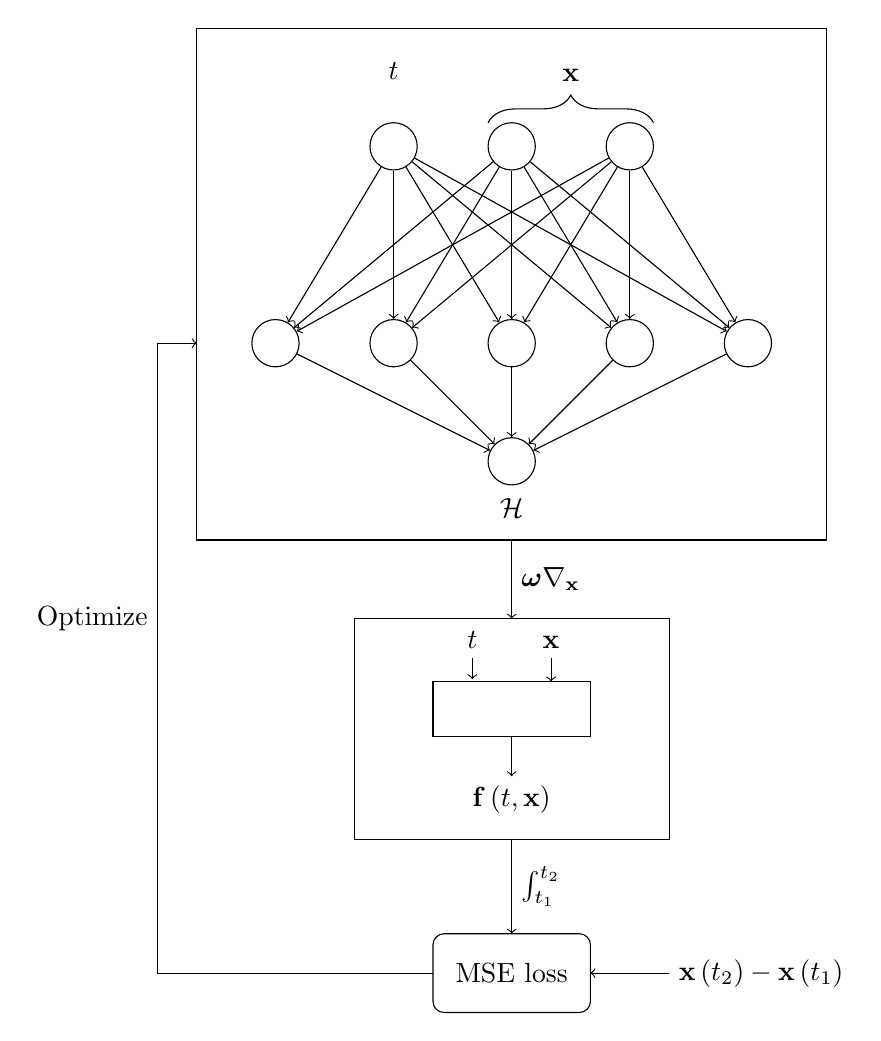
\begin{tikzpicture}
		\tikzstyle{neuron}=[circle,draw=black,minimum size=0.6cm,inner sep=0]
		\foreach \x in {-1,...,1}
			\node[neuron] (input\x) at (1.5*\x, 0) {};
		\foreach \x in {-2,...,2}
			\node[neuron] (hidden\x) at (1.5*\x, -2.5) {};
		\node[neuron] (output) at (0, -4) {};

		\foreach \xin in {-1,...,1}
			\foreach \xout in {-2,...,2}
				\path[->] (input\xin) edge (hidden\xout);
		\foreach \xin in {-2,...,2}
			\path[->] (hidden\xin) edge (output);

		\node at (-1.5,0.6cm+10pt) {$t$};
		\draw[decorate,decoration={brace,amplitude=10pt},xshift=0,yshift=0.6cm]
				(-0.3,-0.3) -- (1.8,-0.3) node[midway,yshift=0.6cm] {$\mathbf x$};
		\node at (0,-4.6) {$\mathcal H$};

		\draw (-4,1.5) rectangle (4,-5);
		\draw[->] (0,-5) -- (0,-6) node[midway,anchor=west] {$\boldsymbol\omega\nabla_{\mathbf x}$};

		\draw (-2,-6) rectangle (2,-8.8);
		\node[anchor=south] (tin) at (-0.5,-6.5) {$t$};
		\node[anchor=south] (xin) at (0.5,-6.5) {$\mathbf x$};
		\draw[->] (tin) -- +(0,-0.5);
		\draw[->] (xin) -- +(0,-0.5);
		\draw (-1,-6.8) rectangle (1,-7.5);
		\node[anchor=north] (fout) at (0,-8) {$\mathbf f\left(t,\mathbf x\right)$};
		\draw[->] (0,-7.5) -- (fout);

		\draw[->] (0,-8.8) -- (0,-10) node[midway,anchor=west] {$\int_{t_1}^{t_2}$};
		\draw[rounded corners] (-1,-10) rectangle (1,-11);
		\node at (0,-10.5) {MSE loss};
		\node[anchor=west] (truth) at (2,-10.5) {$\mathbf x\left(t_2\right)-\mathbf x\left(t_1\right)$};
		\draw[->] (truth) -- (1,-10.5);

		\draw[->] (-1,-10.5) -- (-4.5,-10.5) -- (-4.5,-2.5) -- (-4,-2.5);
		\node[anchor=east] at (-4.5,-6) {Optimize};
	\end{tikzpicture}
	\caption{The train circle of a self-supervised hamiltonian neural network}
	\label{fig:selfsup_train}
\end{figure}

\section{The training}
\label{sec:training}

Our goal is to derive the function $\left(t,\mathbf x\right)\mapsto\mathcal H$
according to the dataset containing a series of samples in form of $\left(t,\mathbf x\right)$ on a series of possible motions of the system.
To make our work simpler,
we assume that $\partial\mathcal H/\partial t=0$,
which fits with most cases.

The dataset does not contain the $\dot{\mathbf x}$ infomation,
which acts as the ground truth in the supervised model \cite{greydanus2019hamiltonian}.
Our model is self-supervised, and thus does not need the $\dot{\mathbf x}$ infomation.

The model uses the loss inspired from Equation \ref{eq:int}
\begin{equation}
	\mathcal L:=\operatorname{MSE}\left(\mathbf x\left(t_1\right)+\int_{t_1}^{t_2}\boldsymbol\omega\nabla_{\mathbf x}\mathcal H\mathrm dt,\mathbf x\left(t_2\right)\right),
\end{equation}
where $\left(t_1,\mathbf x\left(t_1\right)\right)$ and $\left(t_1,\mathbf x\left(t_1\right)\right)$
are 2 samples from the same motion of the system.
The complete process of a traning circle is shown in Figure \ref{fig:selfsup_train}.
For comparison, the train circle of the supervised hamiltonian neural network
is shown in Figure \ref{fig:sup_train}.

The Adam optimizer \cite{kingma2017adam} is used for optimizing the neural network.

\section{Few-parameters optimization}

\begin{figure}
	\centering
	\begin{subfigure}[b]{0.4\linewidth}
		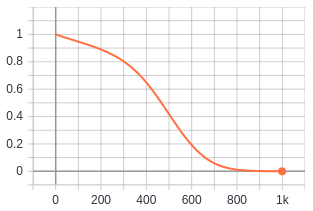
\includegraphics[width=\linewidth]{few_param_loss.png}
		\caption{The change in loss during the training}
	\end{subfigure}
	\begin{subfigure}[b]{0.4\linewidth}
		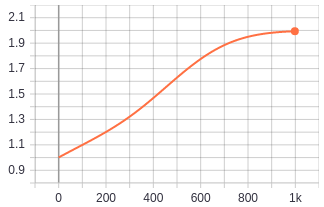
\includegraphics[width=\linewidth]{few_param_omega.png}
		\caption{The change in $\omega$ during the training}
	\end{subfigure}
	\caption{The process of training using the few-parameters optimization (abscissa is the epoch number)}
	\label{fig:few_param}
\end{figure}

\begin{figure}
	\centering
	\begin{subfigure}[b]{0.4\linewidth}
		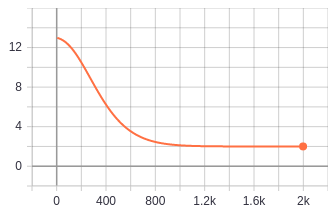
\includegraphics[width=\linewidth]{few_param_loss_bad.png}
		\caption{The change in loss during the training, converging to a non-zero value}
	\end{subfigure}
	\begin{subfigure}[b]{0.4\linewidth}
		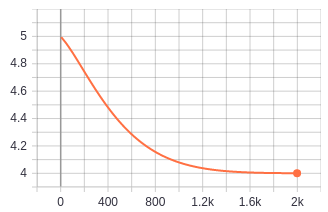
\includegraphics[width=\linewidth]{few_param_omega_bad.png}
		\caption{The change in $\omega$ during the training, converging to a wrong answer}
	\end{subfigure}
	\caption{The process of training using the few-parameters optimization, but coming out with a bad result}
	\label{fig:few_param_bad}
\end{figure}

If the form of the hamiltonian is previously known,
and there are just a few parameters in the formula of the hamiltonian to be decided,
the few-parameters optimization.

For example, there is a harmonic oscillator with its frequency unknown.
Its hamiltonian is
\begin{equation}
	\mathcal H=\frac12p^2+\frac12\omega^2q^2,
\end{equation}
where $\omega$ is the only parameter that should be optimized.

We can use the procedure explained in Section \ref{sec:training}
to optimize the parameter.

Here we have gone on an experiment.
Use the ground truth $\omega=2$, and initialize the parameter as $\omega=1$.
Use a dataset with only 2 datas $\mathbf x\left(0\right)=\left(1,0\right)$,
and $\mathbf x\left(\frac\pi2\right)=\left(-1,0\right)$.
After we trained it for $1000$ epoches with learn rate $\SI{1e-3}{}$,
the parameter is optimized to the true value $2$.

The change in loss and $\omega$ during the training is shown in Figure \ref{fig:few_param}.

Although the few-parameters optimization experiment does not have much value
because we often do not know the form of the hamiltonian before we train the model,
this experiment shows that the method introduced in Section \ref{sec:training} is feasible.

However, this method has some flaw. If we take the initial value of $\omega$ as $5.0$,
the final value of $\omega$ is not correct.
This is because the loss has multiple minimals w.r.t. $\omega$ \cite[p. 121]{reed1999smithing},
one of which is $2$, taken when $\omega=4$.
Specially, in some cases, the wrong minimal of loss can be $0$,
so we cannot judge whether the result of the optimized parameter is correct
by looking at whether the loss is $0$.

This reminds us that the method has its limitations.
To avoid the wrong result, the dataset should be comprehensive enough.
After some trials, we found that the best strategy is to switch to another data
when the loss converges.
After switching the data several times,
the parameters should converge to a correct value.

\section{Tasks}

\subsection{Free particle}

\begin{figure}[h]
	\centering
	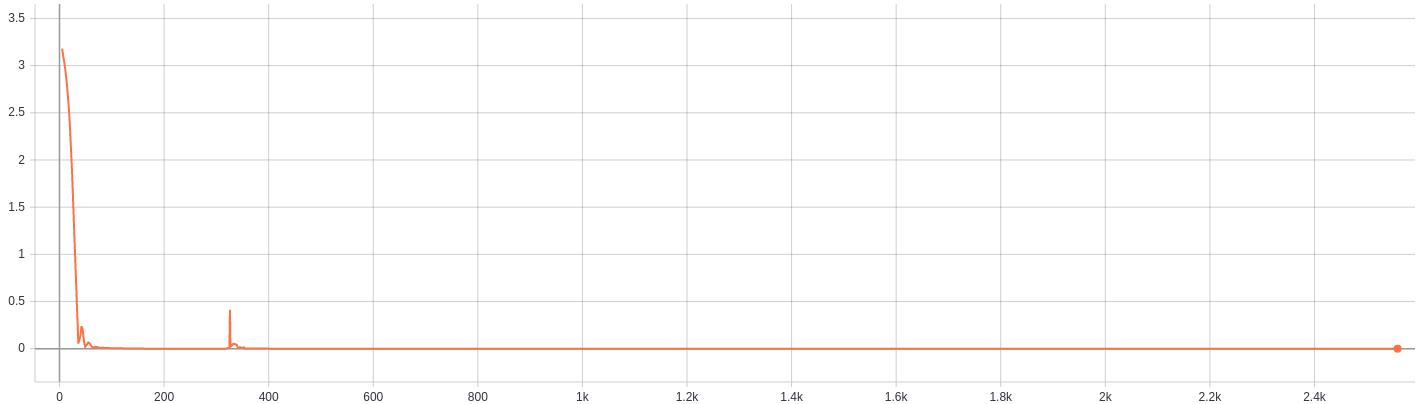
\includegraphics[width=\linewidth]{free_loss.png}
	\caption{The loss change during the training of the model of free particle}
	\label{fig:free_loss}
\end{figure}

A free particle is a system with 1 DOF whose hamiltonian is \cite[p. 133]{landau1976mechanics}\cite[p. 66]{arnold1989mathmech}
\begin{equation*}
	\mathcal H\left(t,q,p\right):=\frac{p^2}{2m},
\end{equation*}
where $m$ is the mass of the particle.
To be simple, we take $m:=1/2$.

The model of a free particle is the simplest model.
We take this model as the first task to test the basic capability of our idea.

The dataset is generated using a ODE solver.
The dataset has totally $16$ datas.
Every data consists of the size of considered time interval
(lies in the range $\left(0,2\right)$),
a series of $200$ different initial conditions
(lies in the range $\left(-1,1\right)^2$)
to be learned as a batch,
and the corresponding state of the system at the end of the time interval.

Every data is learned for $160$ epoches.
When a data is finished, the neural network moves on to the next data.
Thus there are totally $2560$ steps.
The loss change in shown in Figure \ref{fig:free_loss}.

\subsection{Harmonic oscillator}

\begin{figure}[h]
	\centering
	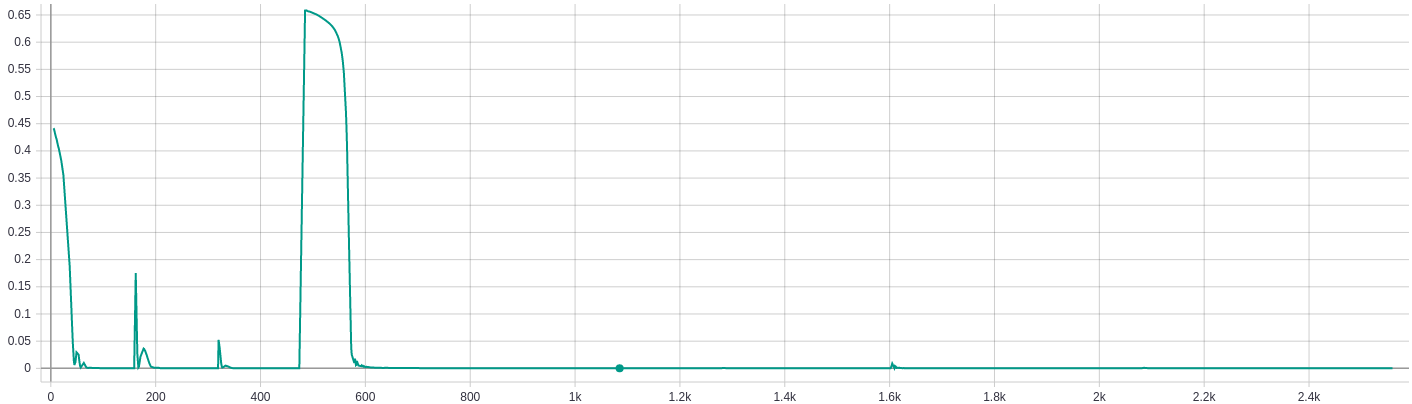
\includegraphics[width=\linewidth]{spring_loss.png}
	\caption{The loss change during the training of the model of a harmonic oscillator}
	\label{fig:spring_loss}
\end{figure}

\begin{figure}[h]
	\centering
	\begin{subfigure}[b]{0.45\linewidth}
		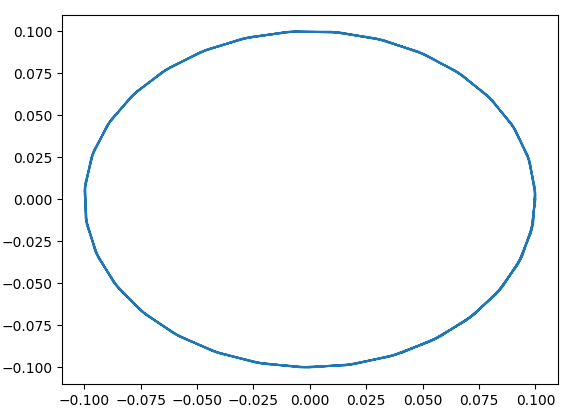
\includegraphics[width=\linewidth]{spring_learned.png}
		\caption{The result given by the trained model}
	\end{subfigure}
	\begin{subfigure}[b]{0.45\linewidth}
		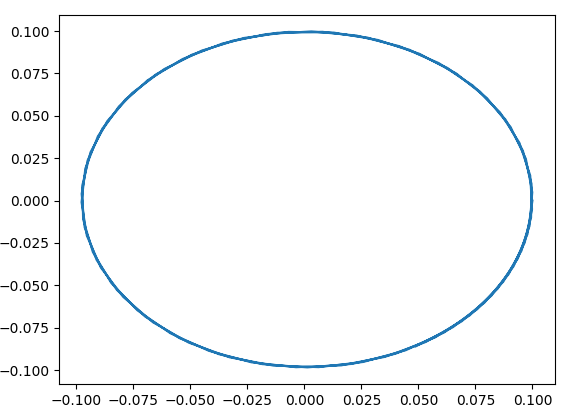
\includegraphics[width=\linewidth]{spring_truth.png}
		\caption{The ground truth}
	\end{subfigure}
	\caption{The comparation of the result given by the trained model and the ground truth}
	\label{fig:spring_comp}
\end{figure}

A harmonic oscillator is a system with 1 DOF whose hamiltonian is \cite[p. 157]{landau1976mechanics}
\begin{equation*}
	\mathcal H\left(t,q,p\right):=\frac{p^2}{2m}+\frac12kq^2,
\end{equation*}
where $m$ is the mass of the particle, and $k$ is a parameter.
To be simple, we take $m:=1/2$ and $k:=2$.

The dataset is generated using a ODE solver.
The dataset has totally $16$ datas.
Every data consists of the size of considered time interval
(lies in the range $\left(0,2\right)$),
a series of $200$ different initial conditions
(lies in the range $\left(-0.71,0.71\right)^2$)
to be learned as a batch,
and the corresponding state of the system at the end of the time interval.

Every data is learned for $160$ epoches.
When a data is finished, the neural network moves on to the next data.
Thus there are totally $2560$ steps.
The loss change in shown in Figure \ref{fig:spring_loss}.

The loss may suddenly jump to a high value when the neural network switches to a different data
because it may have converged to a wrong minimal of loss when it learns with the last data.

Taking the initial condition $\mathbf x=\left(0.1,0\right)$
to test the trained model and compare it with the ground truth,
the result can be seen in Figure \ref{fig:spring_comp}.
The figure shows the trajectory of the motion in space of $\mathbf x$,
which is the phase path \cite[p. 146]{landau1976mechanics}\cite[p. 68]{arnold1989mathmech}.
As can be seen, it can give the correct result:
the phase path is a circle \cite[p. 17]{arnold1989mathmech}.

\subsection{Kepler's problem}

The Kepler's problem is the motion of a particle in Coulomb field.
Its hamiltonian is
\begin{equation*}
	\mathcal H\left(t,q,p\right):=\frac{p_0^2+p_1^2}{2m}-\frac\alpha{\sqrt{q_0^2+q_1^2}}.
\end{equation*}
To be simple, we take $m:=\frac12$ and $\alpha:=1$.

\bibliographystyle{abbrv}
\bibliography{selfsup_hnn}

\end{document}
